\documentclass[]{article}
\usepackage{lmodern}
\usepackage{amssymb,amsmath}
\usepackage{ifxetex,ifluatex}
\usepackage{fixltx2e} % provides \textsubscript
\ifnum 0\ifxetex 1\fi\ifluatex 1\fi=0 % if pdftex
  \usepackage[T1]{fontenc}
  \usepackage[utf8]{inputenc}
\else % if luatex or xelatex
  \ifxetex
    \usepackage{mathspec}
  \else
    \usepackage{fontspec}
  \fi
  \defaultfontfeatures{Ligatures=TeX,Scale=MatchLowercase}
\fi
% use upquote if available, for straight quotes in verbatim environments
\IfFileExists{upquote.sty}{\usepackage{upquote}}{}
% use microtype if available
\IfFileExists{microtype.sty}{%
\usepackage{microtype}
\UseMicrotypeSet[protrusion]{basicmath} % disable protrusion for tt fonts
}{}
\usepackage[margin=1in]{geometry}
\usepackage{hyperref}
\hypersetup{unicode=true,
            pdftitle={Project 4 : Explartion of Red Wine Quality},
            pdfauthor={Isabel María Villalba Jiménez},
            pdfborder={0 0 0},
            breaklinks=true}
\urlstyle{same}  % don't use monospace font for urls
\usepackage{natbib}
\bibliographystyle{apsr}
\usepackage{color}
\usepackage{fancyvrb}
\newcommand{\VerbBar}{|}
\newcommand{\VERB}{\Verb[commandchars=\\\{\}]}
\DefineVerbatimEnvironment{Highlighting}{Verbatim}{commandchars=\\\{\}}
% Add ',fontsize=\small' for more characters per line
\usepackage{framed}
\definecolor{shadecolor}{RGB}{248,248,248}
\newenvironment{Shaded}{\begin{snugshade}}{\end{snugshade}}
\newcommand{\KeywordTok}[1]{\textcolor[rgb]{0.13,0.29,0.53}{\textbf{{#1}}}}
\newcommand{\DataTypeTok}[1]{\textcolor[rgb]{0.13,0.29,0.53}{{#1}}}
\newcommand{\DecValTok}[1]{\textcolor[rgb]{0.00,0.00,0.81}{{#1}}}
\newcommand{\BaseNTok}[1]{\textcolor[rgb]{0.00,0.00,0.81}{{#1}}}
\newcommand{\FloatTok}[1]{\textcolor[rgb]{0.00,0.00,0.81}{{#1}}}
\newcommand{\ConstantTok}[1]{\textcolor[rgb]{0.00,0.00,0.00}{{#1}}}
\newcommand{\CharTok}[1]{\textcolor[rgb]{0.31,0.60,0.02}{{#1}}}
\newcommand{\SpecialCharTok}[1]{\textcolor[rgb]{0.00,0.00,0.00}{{#1}}}
\newcommand{\StringTok}[1]{\textcolor[rgb]{0.31,0.60,0.02}{{#1}}}
\newcommand{\VerbatimStringTok}[1]{\textcolor[rgb]{0.31,0.60,0.02}{{#1}}}
\newcommand{\SpecialStringTok}[1]{\textcolor[rgb]{0.31,0.60,0.02}{{#1}}}
\newcommand{\ImportTok}[1]{{#1}}
\newcommand{\CommentTok}[1]{\textcolor[rgb]{0.56,0.35,0.01}{\textit{{#1}}}}
\newcommand{\DocumentationTok}[1]{\textcolor[rgb]{0.56,0.35,0.01}{\textbf{\textit{{#1}}}}}
\newcommand{\AnnotationTok}[1]{\textcolor[rgb]{0.56,0.35,0.01}{\textbf{\textit{{#1}}}}}
\newcommand{\CommentVarTok}[1]{\textcolor[rgb]{0.56,0.35,0.01}{\textbf{\textit{{#1}}}}}
\newcommand{\OtherTok}[1]{\textcolor[rgb]{0.56,0.35,0.01}{{#1}}}
\newcommand{\FunctionTok}[1]{\textcolor[rgb]{0.00,0.00,0.00}{{#1}}}
\newcommand{\VariableTok}[1]{\textcolor[rgb]{0.00,0.00,0.00}{{#1}}}
\newcommand{\ControlFlowTok}[1]{\textcolor[rgb]{0.13,0.29,0.53}{\textbf{{#1}}}}
\newcommand{\OperatorTok}[1]{\textcolor[rgb]{0.81,0.36,0.00}{\textbf{{#1}}}}
\newcommand{\BuiltInTok}[1]{{#1}}
\newcommand{\ExtensionTok}[1]{{#1}}
\newcommand{\PreprocessorTok}[1]{\textcolor[rgb]{0.56,0.35,0.01}{\textit{{#1}}}}
\newcommand{\AttributeTok}[1]{\textcolor[rgb]{0.77,0.63,0.00}{{#1}}}
\newcommand{\RegionMarkerTok}[1]{{#1}}
\newcommand{\InformationTok}[1]{\textcolor[rgb]{0.56,0.35,0.01}{\textbf{\textit{{#1}}}}}
\newcommand{\WarningTok}[1]{\textcolor[rgb]{0.56,0.35,0.01}{\textbf{\textit{{#1}}}}}
\newcommand{\AlertTok}[1]{\textcolor[rgb]{0.94,0.16,0.16}{{#1}}}
\newcommand{\ErrorTok}[1]{\textcolor[rgb]{0.64,0.00,0.00}{\textbf{{#1}}}}
\newcommand{\NormalTok}[1]{{#1}}
\usepackage{graphicx,grffile}
\makeatletter
\def\maxwidth{\ifdim\Gin@nat@width>\linewidth\linewidth\else\Gin@nat@width\fi}
\def\maxheight{\ifdim\Gin@nat@height>\textheight\textheight\else\Gin@nat@height\fi}
\makeatother
% Scale images if necessary, so that they will not overflow the page
% margins by default, and it is still possible to overwrite the defaults
% using explicit options in \includegraphics[width, height, ...]{}
\setkeys{Gin}{width=\maxwidth,height=\maxheight,keepaspectratio}
\IfFileExists{parskip.sty}{%
\usepackage{parskip}
}{% else
\setlength{\parindent}{0pt}
\setlength{\parskip}{6pt plus 2pt minus 1pt}
}
\setlength{\emergencystretch}{3em}  % prevent overfull lines
\providecommand{\tightlist}{%
  \setlength{\itemsep}{0pt}\setlength{\parskip}{0pt}}
\setcounter{secnumdepth}{0}
% Redefines (sub)paragraphs to behave more like sections
\ifx\paragraph\undefined\else
\let\oldparagraph\paragraph
\renewcommand{\paragraph}[1]{\oldparagraph{#1}\mbox{}}
\fi
\ifx\subparagraph\undefined\else
\let\oldsubparagraph\subparagraph
\renewcommand{\subparagraph}[1]{\oldsubparagraph{#1}\mbox{}}
\fi

%%% Use protect on footnotes to avoid problems with footnotes in titles
\let\rmarkdownfootnote\footnote%
\def\footnote{\protect\rmarkdownfootnote}

%%% Change title format to be more compact
\usepackage{titling}

% Create subtitle command for use in maketitle
\newcommand{\subtitle}[1]{
  \posttitle{
    \begin{center}\large#1\end{center}
    }
}

\setlength{\droptitle}{-2em}
  \title{Project 4 : Explartion of Red Wine Quality}
  \pretitle{\vspace{\droptitle}\centering\huge}
  \posttitle{\par}
  \author{Isabel María Villalba Jiménez}
  \preauthor{\centering\large\emph}
  \postauthor{\par}
  \predate{\centering\large\emph}
  \postdate{\par}
  \date{December 6th, 2016}


\begin{document}
\maketitle

\section{Analysis}\label{analysis}

In this work it will be analyzed the impact in quality of several
parameters describing red wine. The dataset is curated by Udacity and
comes from UCI repository
\url{https://archive.ics.uci.edu/ml/datasets/Wine+Quality} and consists
of 1599 sample data for Red wine
\url{https://docs.google.com/document/d/1qEcwltBMlRYZT-l699-71TzInWfk4W9q5rTCSvDVMpc/pub?embedded=true}.

In \citet{cortez2009modeling} it is shown that the most imporant
features for assessing Red Wine quality are:

\begin{itemize}
\item
  sulphates
\item
  pH
\item
  total sulfur dioxide
\end{itemize}

\section{Variable summary}\label{variable-summary}

\begin{Shaded}
\begin{Highlighting}[]
\CommentTok{# Load the Data}
\NormalTok{redwines <-}\StringTok{ }\KeywordTok{read.csv}\NormalTok{(}\StringTok{'wineQualityReds.csv'}\NormalTok{)}

\KeywordTok{dim}\NormalTok{(redwines)}
\end{Highlighting}
\end{Shaded}

\begin{verbatim}
## [1] 1599   13
\end{verbatim}

\begin{Shaded}
\begin{Highlighting}[]
\CommentTok{#names(redwines)}
\KeywordTok{summary}\NormalTok{(redwines)}
\end{Highlighting}
\end{Shaded}

\begin{verbatim}
##        X          fixed.acidity   volatile.acidity  citric.acid   
##  Min.   :   1.0   Min.   : 4.60   Min.   :0.1200   Min.   :0.000  
##  1st Qu.: 400.5   1st Qu.: 7.10   1st Qu.:0.3900   1st Qu.:0.090  
##  Median : 800.0   Median : 7.90   Median :0.5200   Median :0.260  
##  Mean   : 800.0   Mean   : 8.32   Mean   :0.5278   Mean   :0.271  
##  3rd Qu.:1199.5   3rd Qu.: 9.20   3rd Qu.:0.6400   3rd Qu.:0.420  
##  Max.   :1599.0   Max.   :15.90   Max.   :1.5800   Max.   :1.000  
##  residual.sugar     chlorides       free.sulfur.dioxide
##  Min.   : 0.900   Min.   :0.01200   Min.   : 1.00      
##  1st Qu.: 1.900   1st Qu.:0.07000   1st Qu.: 7.00      
##  Median : 2.200   Median :0.07900   Median :14.00      
##  Mean   : 2.539   Mean   :0.08747   Mean   :15.87      
##  3rd Qu.: 2.600   3rd Qu.:0.09000   3rd Qu.:21.00      
##  Max.   :15.500   Max.   :0.61100   Max.   :72.00      
##  total.sulfur.dioxide    density             pH          sulphates     
##  Min.   :  6.00       Min.   :0.9901   Min.   :2.740   Min.   :0.3300  
##  1st Qu.: 22.00       1st Qu.:0.9956   1st Qu.:3.210   1st Qu.:0.5500  
##  Median : 38.00       Median :0.9968   Median :3.310   Median :0.6200  
##  Mean   : 46.47       Mean   :0.9967   Mean   :3.311   Mean   :0.6581  
##  3rd Qu.: 62.00       3rd Qu.:0.9978   3rd Qu.:3.400   3rd Qu.:0.7300  
##  Max.   :289.00       Max.   :1.0037   Max.   :4.010   Max.   :2.0000  
##     alcohol         quality     
##  Min.   : 8.40   Min.   :3.000  
##  1st Qu.: 9.50   1st Qu.:5.000  
##  Median :10.20   Median :6.000  
##  Mean   :10.42   Mean   :5.636  
##  3rd Qu.:11.10   3rd Qu.:6.000  
##  Max.   :14.90   Max.   :8.000
\end{verbatim}

\begin{Shaded}
\begin{Highlighting}[]
\CommentTok{# New variables }
\CommentTok{#redwines$quality.factor <- factor(redwines$quality)}

\NormalTok{redwines$quality.cat <-}\StringTok{ }\OtherTok{NA}
\NormalTok{redwines$quality.cat <-}\StringTok{ }\KeywordTok{ifelse}\NormalTok{(redwines$quality>=}\DecValTok{7}\NormalTok{, }\StringTok{'good'}\NormalTok{,}\StringTok{'medium'}\NormalTok{)}
\NormalTok{redwines$quality.cat <-}\StringTok{ }\KeywordTok{ifelse}\NormalTok{(redwines$quality<=}\DecValTok{4}\NormalTok{, }\StringTok{'bad'}\NormalTok{,redwines$quality.cat) }\CommentTok{# if not, leave the previous values}
\NormalTok{redwines$quality.cat <-}\StringTok{ }\KeywordTok{factor}\NormalTok{(redwines$quality.cat, }\DataTypeTok{levels =} \KeywordTok{list}\NormalTok{(}\StringTok{'bad'}\NormalTok{, }\StringTok{'medium'}\NormalTok{,}\StringTok{'good'}\NormalTok{)) }\CommentTok{# set the order!}

\KeywordTok{print}\NormalTok{(}\StringTok{"Variables after dividing into quality groups"}\NormalTok{)}
\end{Highlighting}
\end{Shaded}

\begin{verbatim}
## [1] "Variables after dividing into quality groups"
\end{verbatim}

\begin{Shaded}
\begin{Highlighting}[]
\KeywordTok{str}\NormalTok{(redwines) }\CommentTok{#summary of values for each variable}
\end{Highlighting}
\end{Shaded}

\begin{verbatim}
## 'data.frame':    1599 obs. of  14 variables:
##  $ X                   : int  1 2 3 4 5 6 7 8 9 10 ...
##  $ fixed.acidity       : num  7.4 7.8 7.8 11.2 7.4 7.4 7.9 7.3 7.8 7.5 ...
##  $ volatile.acidity    : num  0.7 0.88 0.76 0.28 0.7 0.66 0.6 0.65 0.58 0.5 ...
##  $ citric.acid         : num  0 0 0.04 0.56 0 0 0.06 0 0.02 0.36 ...
##  $ residual.sugar      : num  1.9 2.6 2.3 1.9 1.9 1.8 1.6 1.2 2 6.1 ...
##  $ chlorides           : num  0.076 0.098 0.092 0.075 0.076 0.075 0.069 0.065 0.073 0.071 ...
##  $ free.sulfur.dioxide : num  11 25 15 17 11 13 15 15 9 17 ...
##  $ total.sulfur.dioxide: num  34 67 54 60 34 40 59 21 18 102 ...
##  $ density             : num  0.998 0.997 0.997 0.998 0.998 ...
##  $ pH                  : num  3.51 3.2 3.26 3.16 3.51 3.51 3.3 3.39 3.36 3.35 ...
##  $ sulphates           : num  0.56 0.68 0.65 0.58 0.56 0.56 0.46 0.47 0.57 0.8 ...
##  $ alcohol             : num  9.4 9.8 9.8 9.8 9.4 9.4 9.4 10 9.5 10.5 ...
##  $ quality             : int  5 5 5 6 5 5 5 7 7 5 ...
##  $ quality.cat         : Factor w/ 3 levels "bad","medium",..: 2 2 2 2 2 2 2 3 3 2 ...
\end{verbatim}

\begin{Shaded}
\begin{Highlighting}[]
\CommentTok{#unique(redwines$quality.cat)}
\end{Highlighting}
\end{Shaded}

\subsection{Univariate Plots Section}\label{univariate-plots-section}

In this section it will be analyzed each of the variables describing the
wines.

\subsubsection{Quality}\label{quality}

\begin{quote}
The distribution of wine shows that most of wines have a quality between
5-6 points.
\end{quote}

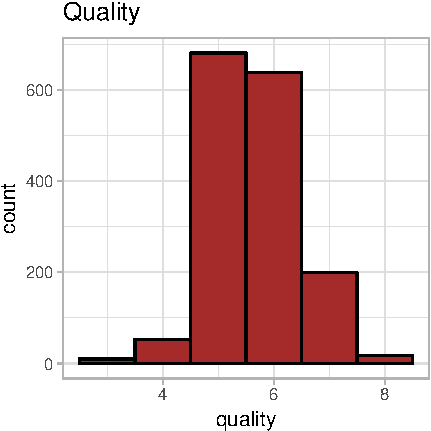
\includegraphics{Figs/Univariate_Plots-1.pdf}

\subsubsection{Fixed and volatile
acidity}\label{fixed-and-volatile-acidity}

\begin{quote}
In the next plot it is deduced that the quality of the wine is directly
proportional to the fixed acidity and acid levels and inversely
proportional to volatile acidity.
\end{quote}

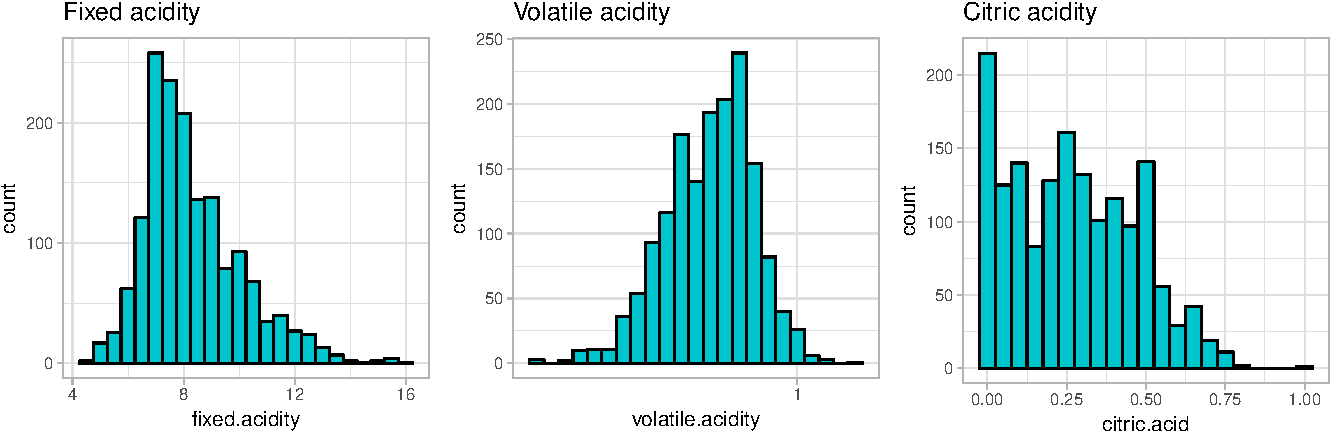
\includegraphics{Figs/Univariate_Plots_acidity-1.pdf}

\subsubsection{Residual sugar}\label{residual-sugar}

\begin{quote}
The plot of residual suggar shows that the better the wine the higher
the residual sugar levels.
\end{quote}

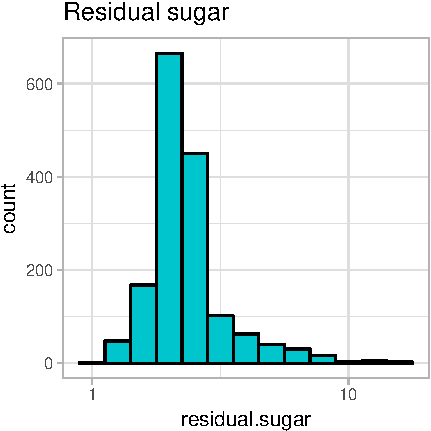
\includegraphics{Figs/Univariate_Plots_residual_sugar-1.pdf}

\subsubsection{Chlorides and sulfur
dioxide}\label{chlorides-and-sulfur-dioxide}

\begin{quote}
In the plot of the chlorides, it can be onserved that the better the
wine, the lower the chloride levels. For the sulfur dioxide, either the
free or the total sulfur dioxide, high levels are indicator of medium
quality, whereas bad and good wine have the same low amount of sulfure
dioxide.
\end{quote}

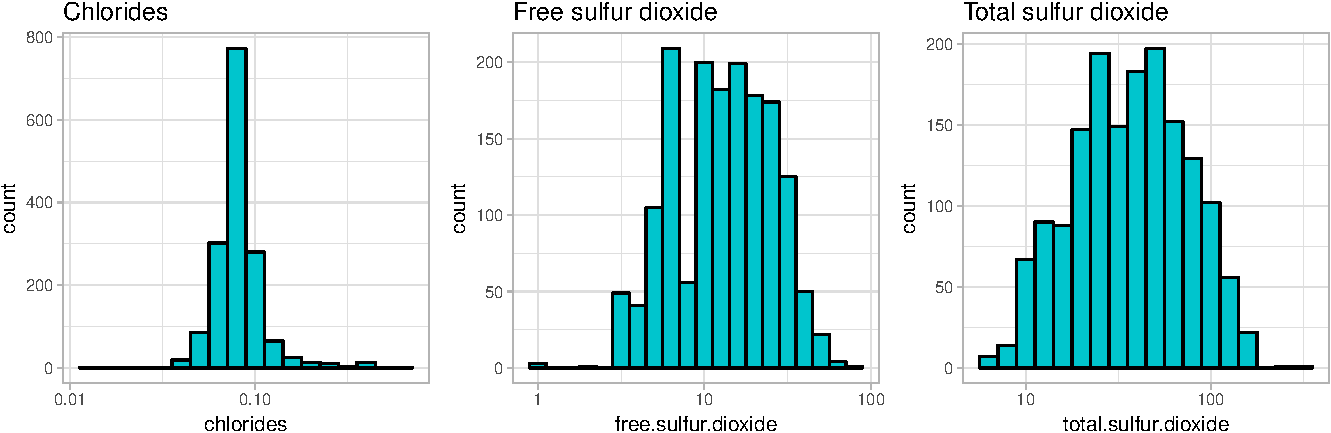
\includegraphics{Figs/Univariate_Plots_chlorides-1.pdf}

\subsubsection{Density, pH, sulphates and
alcohol}\label{density-ph-sulphates-and-alcohol}

\begin{quote}
The next plot shows that, generally, the lower the density, the better
the quality of the wine. ALso, low pH levels are sign of beter quality.
The higher the sulphates level, the better quality of the wine and also,
good wines have higher amount of alcohol.
\end{quote}

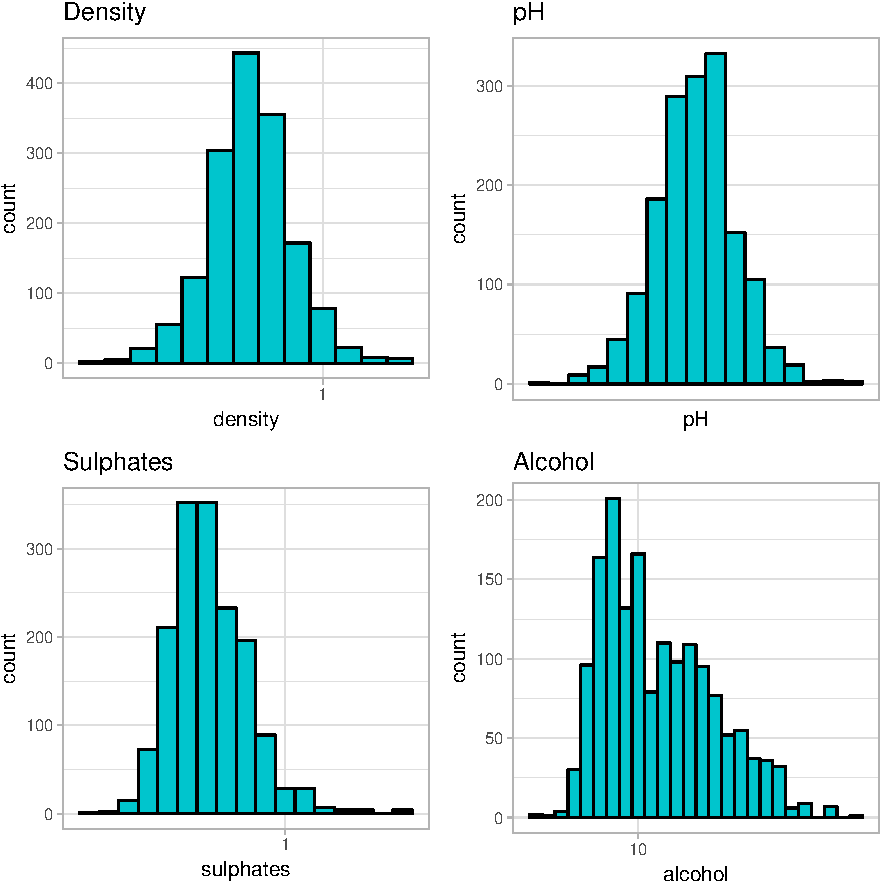
\includegraphics{Figs/Univariate_Plots_density-1.pdf}

\section{Univariate Analysis}\label{univariate-analysis}

\subsubsection{What is the structure of your
dataset?}\label{what-is-the-structure-of-your-dataset}

There are 1599 red wines with 12 features (fixed.acidity,
volatile.acidity, citric.acid, residual.sugar, chlorides,
free.sulfur.dioxide, total.sulfur.dioxide, density, pH, sulphates,
alcohol and quality). The variables quality is converted in a factor
variable (adding a new variable named \texttt{quality.cat}) with the
following levels:

(worst) ----------------\textgreater{} (best)

\texttt{quality.cat}: BAD (quality {[}0,4{]}), MEDIUM (quality (4,7)),
GOOD (quality {[}7,10{]}),

Other observations:

The mean quality of the red wines is 5.636 and the median is 6. Q1
corresponds to 5 and Q3 to 6, hence, 50\% of the data lays within 5-6
range of quality, this is the level MEDIUM.

\subsubsection{What is/are the main feature(s) of interest in your
dataset?}\label{what-isare-the-main-features-of-interest-in-your-dataset}

The main feature of interest in this dataset is the \textbf{quality} of
the wine.

\subsubsection{What other features in the dataset do you think will help
support your investigation into your feature(s) of
interest?}\label{what-other-features-in-the-dataset-do-you-think-will-help-support-your-investigation-into-your-features-of-interest}

In \citet{cortez2009modeling} it is shown that the most imporant
features for assessing Red Wine quality are: \textbf{sulphates},
\textbf{pH} and \textbf{total sulfur dioxide}.

\subsubsection{Did you create any new variables from existing variables
in the
dataset?}\label{did-you-create-any-new-variables-from-existing-variables-in-the-dataset}

The amount of information available is enough to assess the quality of
the wine and I did not create any new variables to support the analysis.

\subsubsection{Of the features you investigated, were there any unusual
distributions? Did you perform any operations on the data to tidy,
adjust, or change the form of the data? If so, why did you do
this?}\label{of-the-features-you-investigated-were-there-any-unusual-distributions-did-you-perform-any-operations-on-the-data-to-tidy-adjust-or-change-the-form-of-the-data-if-so-why-did-you-do-this}

Most of the features had a normal distribution. Some of the features had
quite skewed distributions and many oultiers and I performed a log10
tranformation in order to have a better view.

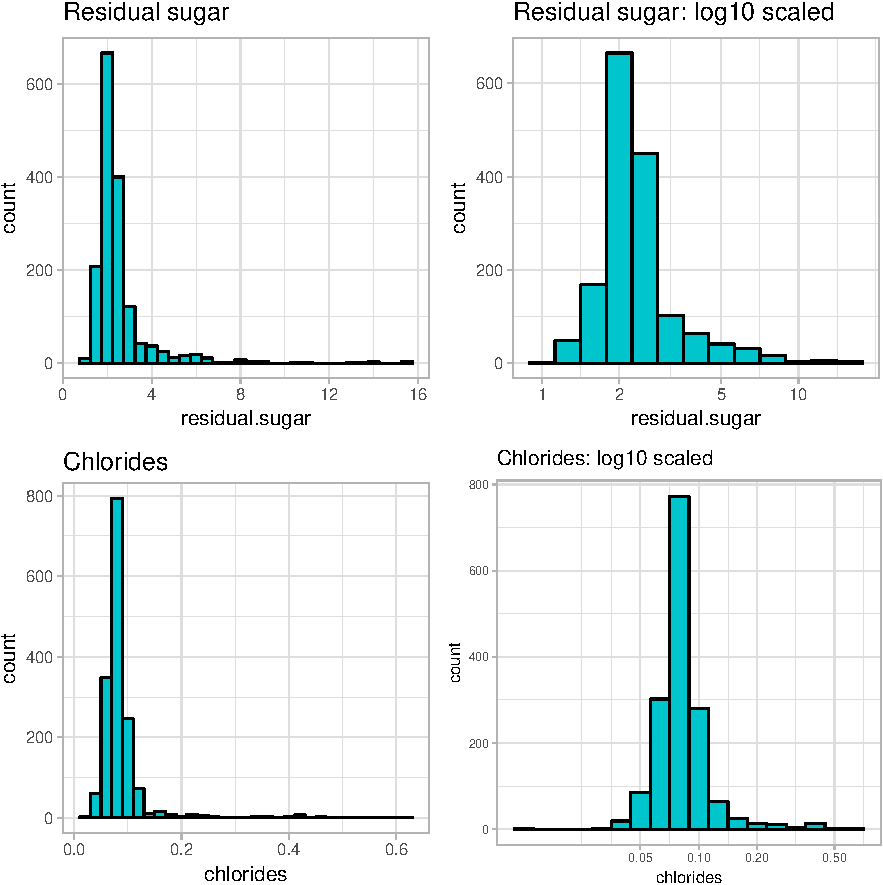
\includegraphics{Figs/univariate_tranformation-1.pdf}

\section{Bivariate Plots Section}\label{bivariate-plots-section}

\subsubsection{Fixed and volatile
acidity}\label{fixed-and-volatile-acidity-1}

\begin{quote}
In the next plot it is deduced that the quality of the wine is directly
proportional to the fixed acidity and acid levels and inversely
proportional to volatile acidity.
\end{quote}

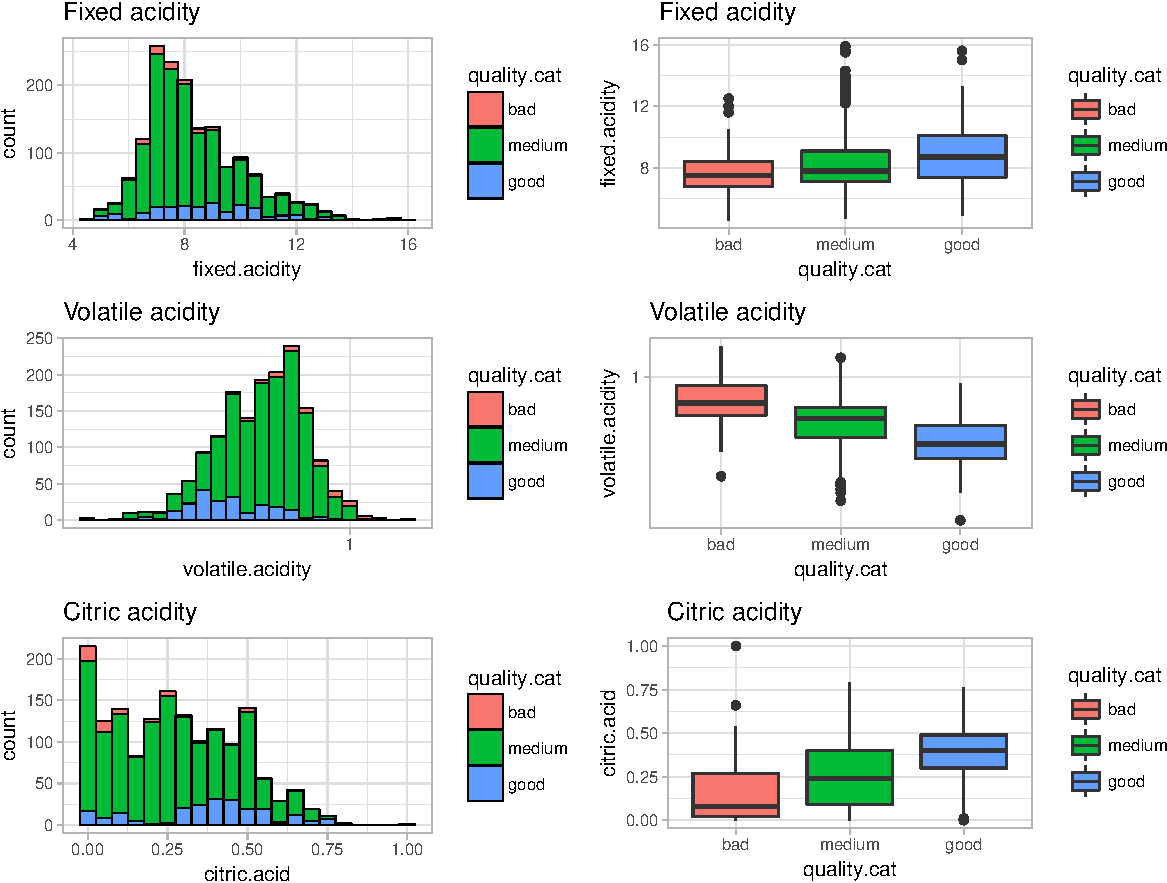
\includegraphics{Figs/Bivariate_Plots_acidity-1.pdf}

\subsubsection{Residual sugar}\label{residual-sugar-1}

\begin{quote}
The plot of residual suggar shows that the better the wine the higher
the residual sugar levels.
\end{quote}

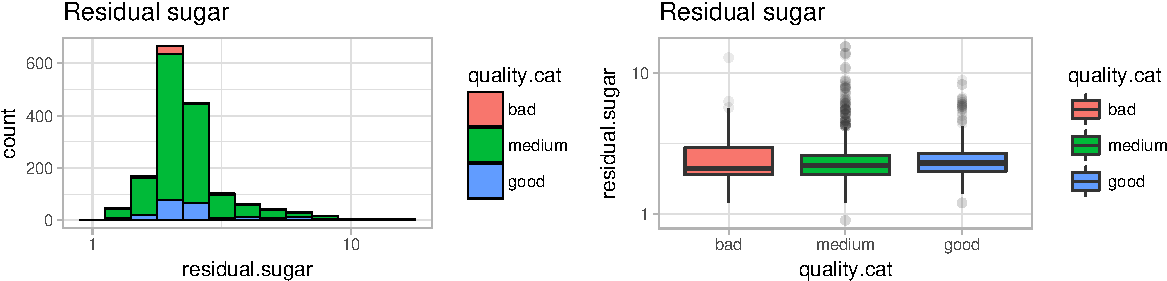
\includegraphics{Figs/Bivariate_Plots_residual_sugar-1.pdf}

\subsubsection{Chlorides and sulfur
dioxide}\label{chlorides-and-sulfur-dioxide-1}

\begin{quote}
In the plot of the chlorides, it can be onserved that the better the
wine, the lower the chloride levels. For the sulfur dioxide, either the
free or the total sulfur dioxide, high levels are indicator of medium
quality, whereas bad and good wine have the same low amount of sulfure
dioxide.
\end{quote}

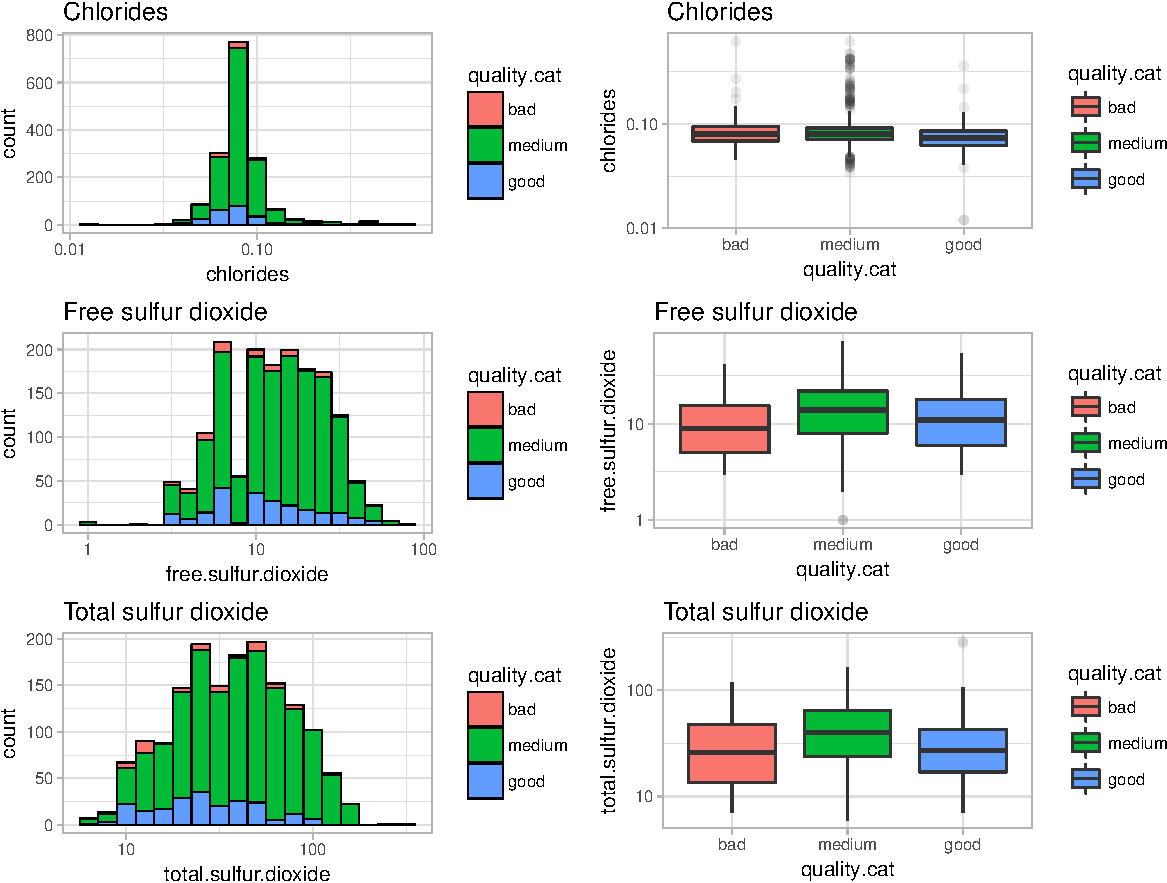
\includegraphics{Figs/Bivariate_Plots_chlorides-1.pdf}

\subsubsection{Density, pH, sulphates and
alcohol}\label{density-ph-sulphates-and-alcohol-1}

\begin{quote}
The next plot shows that, generally, the lower the density, the better
the quality of the wine. ALso, low pH levels are sign of beter quality.
The higher the sulphates level, the better quality of the wine and also,
good wines have higher amount of alcohol.
\end{quote}

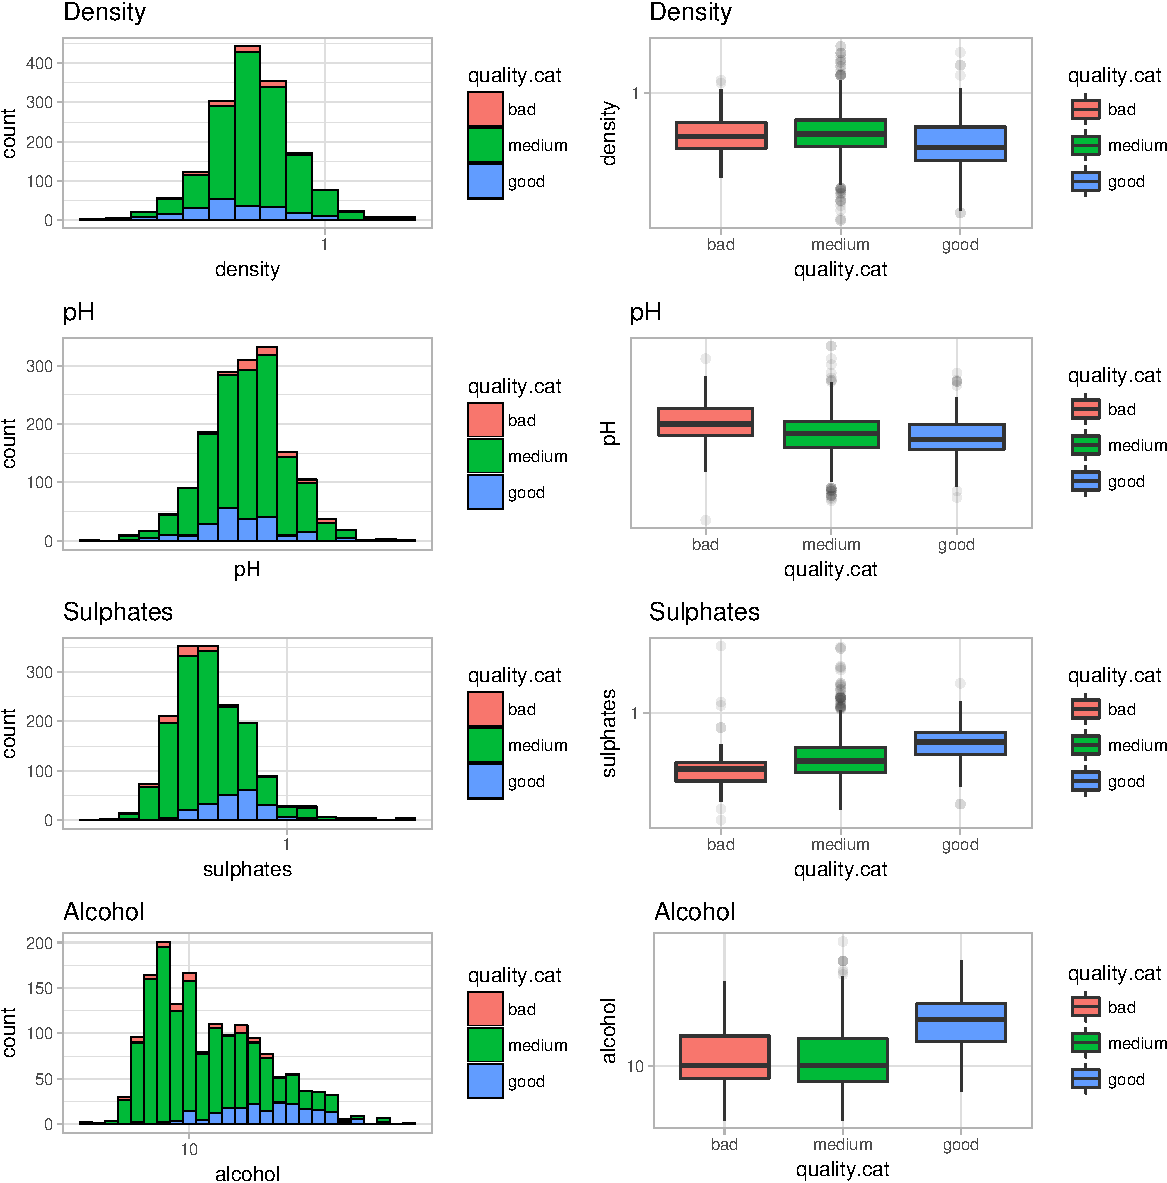
\includegraphics{Figs/Bivariate_Plots_density-1.pdf}

\section{Bivariate Analysis}\label{bivariate-analysis}

\subsubsection{Talk about some of the relationships you observed in this
part of the investigation. How did the feature(s) of interest vary with
other features in the
dataset?}\label{talk-about-some-of-the-relationships-you-observed-in-this-part-of-the-investigation.-how-did-the-features-of-interest-vary-with-other-features-in-the-dataset}

\subsubsection{Did you observe any interesting relationships between the
other features (not the main feature(s) of
interest)?}\label{did-you-observe-any-interesting-relationships-between-the-other-features-not-the-main-features-of-interest}

\subsubsection{What was the strongest relationship you
found?}\label{what-was-the-strongest-relationship-you-found}

\section{Multivariate Plots Section}\label{multivariate-plots-section}

\subsection{Correlation betweeen
variables}\label{correlation-betweeen-variables}

\begin{center}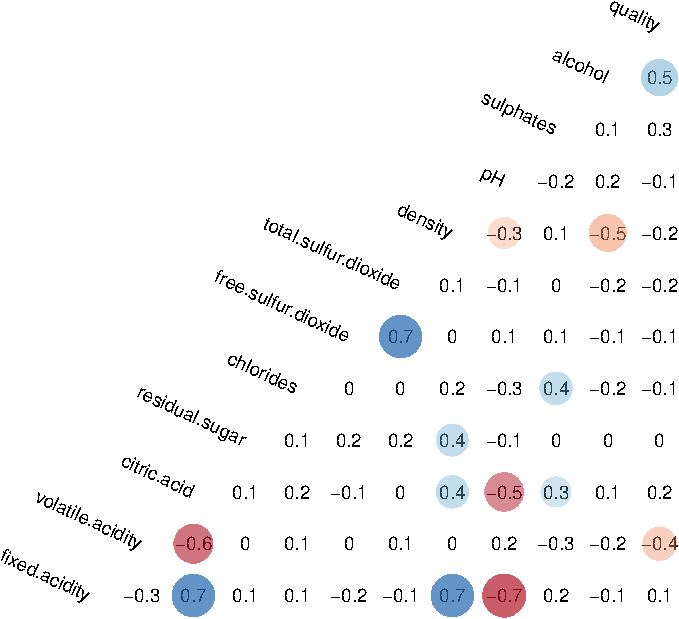
\includegraphics{Figs/Multivariate_Plots_2-1} \end{center}

\subsection{Correlation by quality}\label{correlation-by-quality}

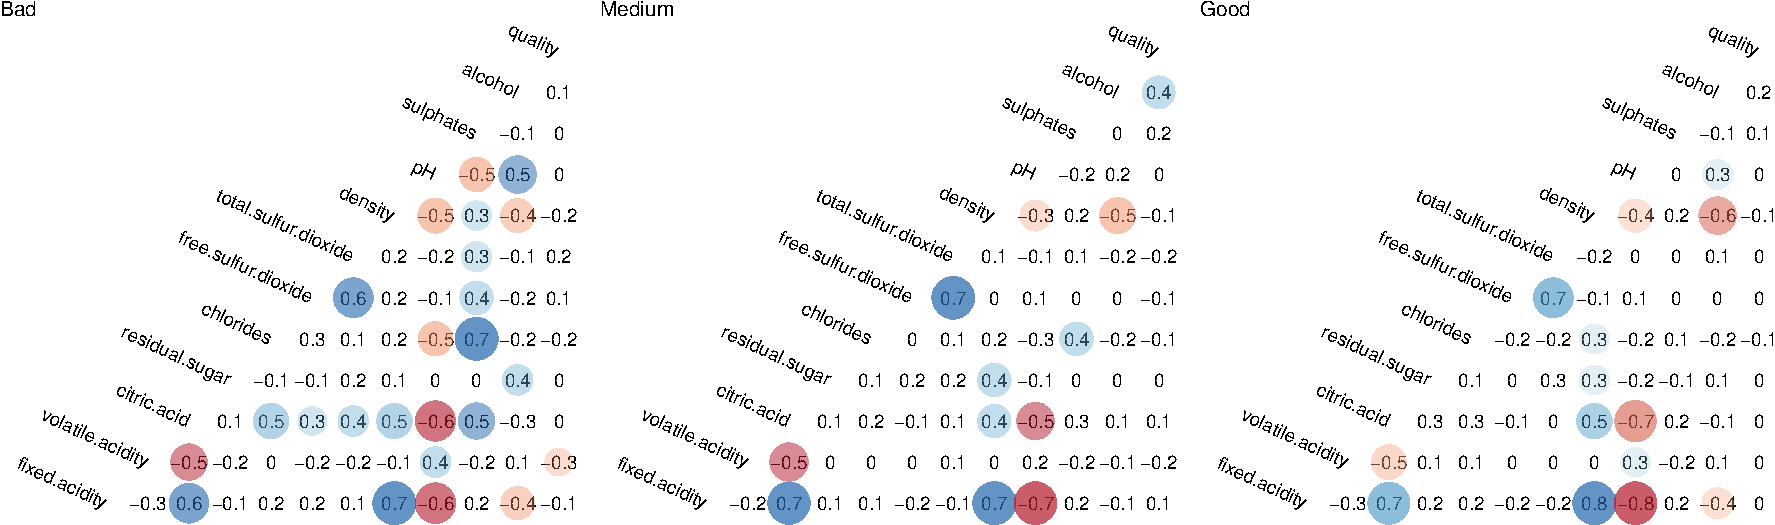
\includegraphics{Figs/unnamed-chunk-2-1.pdf}

From the general correlation matrix, three main variables can be
selected due to their high correlation with quality: \textbf{alcohol}
(R=0.5), \textbf{volatile.acidity} (R=0.4) and \textbf{sulphates}
(R=0.3). In order to see if they are suitable to perform an analysis let
us explore the correlation between them and also the distribution of
samples in bivariates plots in the next graphics
\ref{Correlations_comparative_from_table}.

\begin{figure}

{\centering 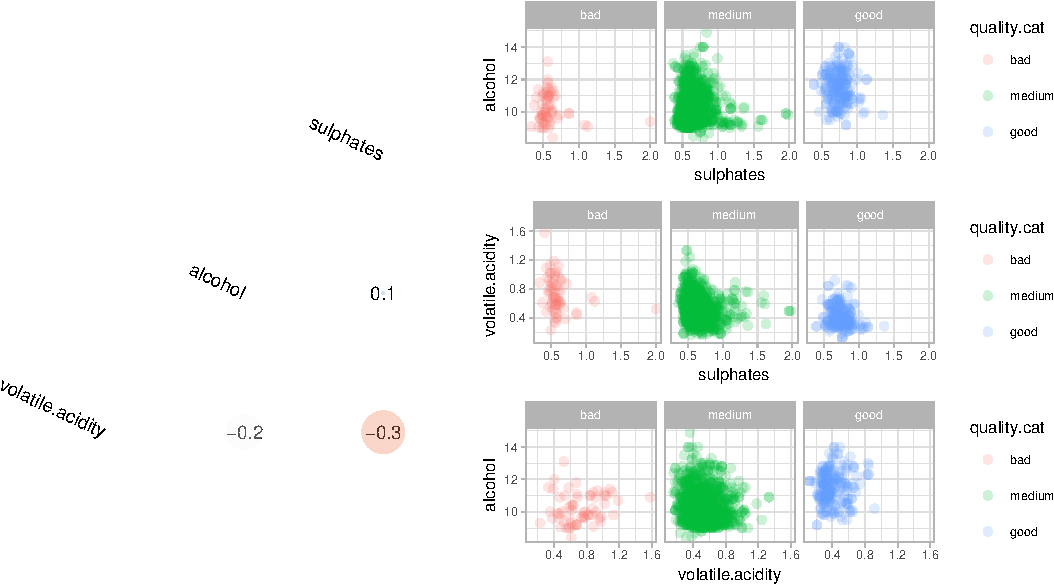
\includegraphics{Figs/Correlations_comparative_from_table-1} 

}

\caption{Correlation between alcohol, volatile acidity and sulphates \label{Correlations_comparative_from_table}}\label{fig:Correlations_comparative_from_table}
\end{figure}

\begin{center}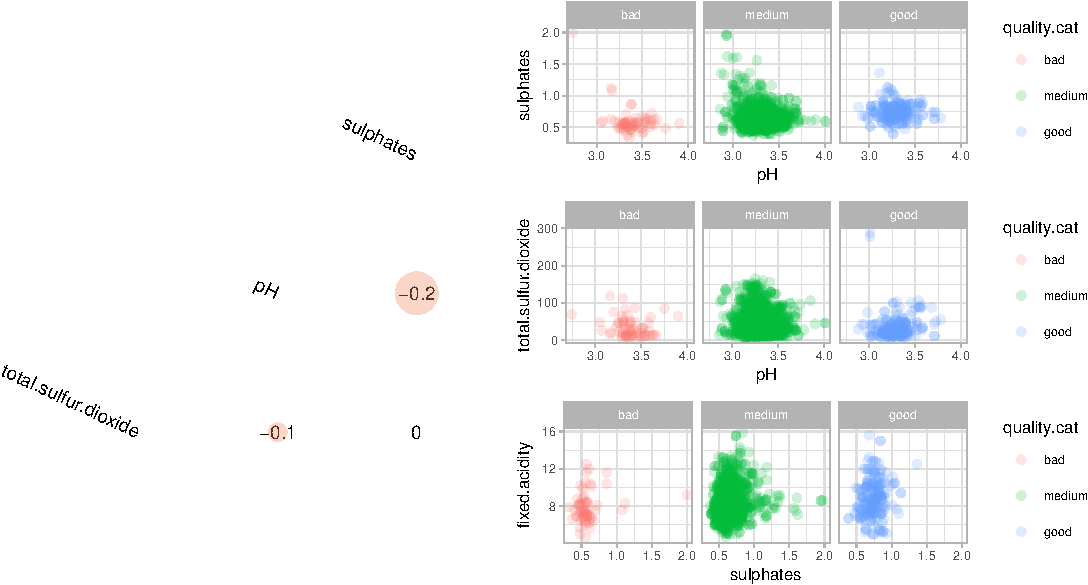
\includegraphics{Figs/Correlations_comparative_from_article-1} \end{center}

\section{Multivariate Analysis}\label{multivariate-analysis}

\subsubsection{Talk about some of the relationships you observed in this
part of the investigation. Were there features that strengthened each
other in terms of looking at your feature(s) of
interest?}\label{talk-about-some-of-the-relationships-you-observed-in-this-part-of-the-investigation.-were-there-features-that-strengthened-each-other-in-terms-of-looking-at-your-features-of-interest}

\subsubsection{Were there any interesting or surprising interactions
between
features?}\label{were-there-any-interesting-or-surprising-interactions-between-features}

\subsubsection{OPTIONAL: Did you create any models with your dataset?
Discuss the strengths and limitations of your
model.}\label{optional-did-you-create-any-models-with-your-dataset-discuss-the-strengths-and-limitations-of-your-model.}

\begin{center}\rule{0.5\linewidth}{\linethickness}\end{center}

\section{Final Plots and Summary}\label{final-plots-and-summary}

\subsubsection{Plot One}\label{plot-one}

\subsubsection{Description One}\label{description-one}

\subsubsection{Plot Two}\label{plot-two}

\subsubsection{Description Two}\label{description-two}

\subsubsection{Plot Three}\label{plot-three}

\subsubsection{Description Three}\label{description-three}

\begin{center}\rule{0.5\linewidth}{\linethickness}\end{center}

\section{Reflection}\label{reflection}

\subsection{References}\label{references}

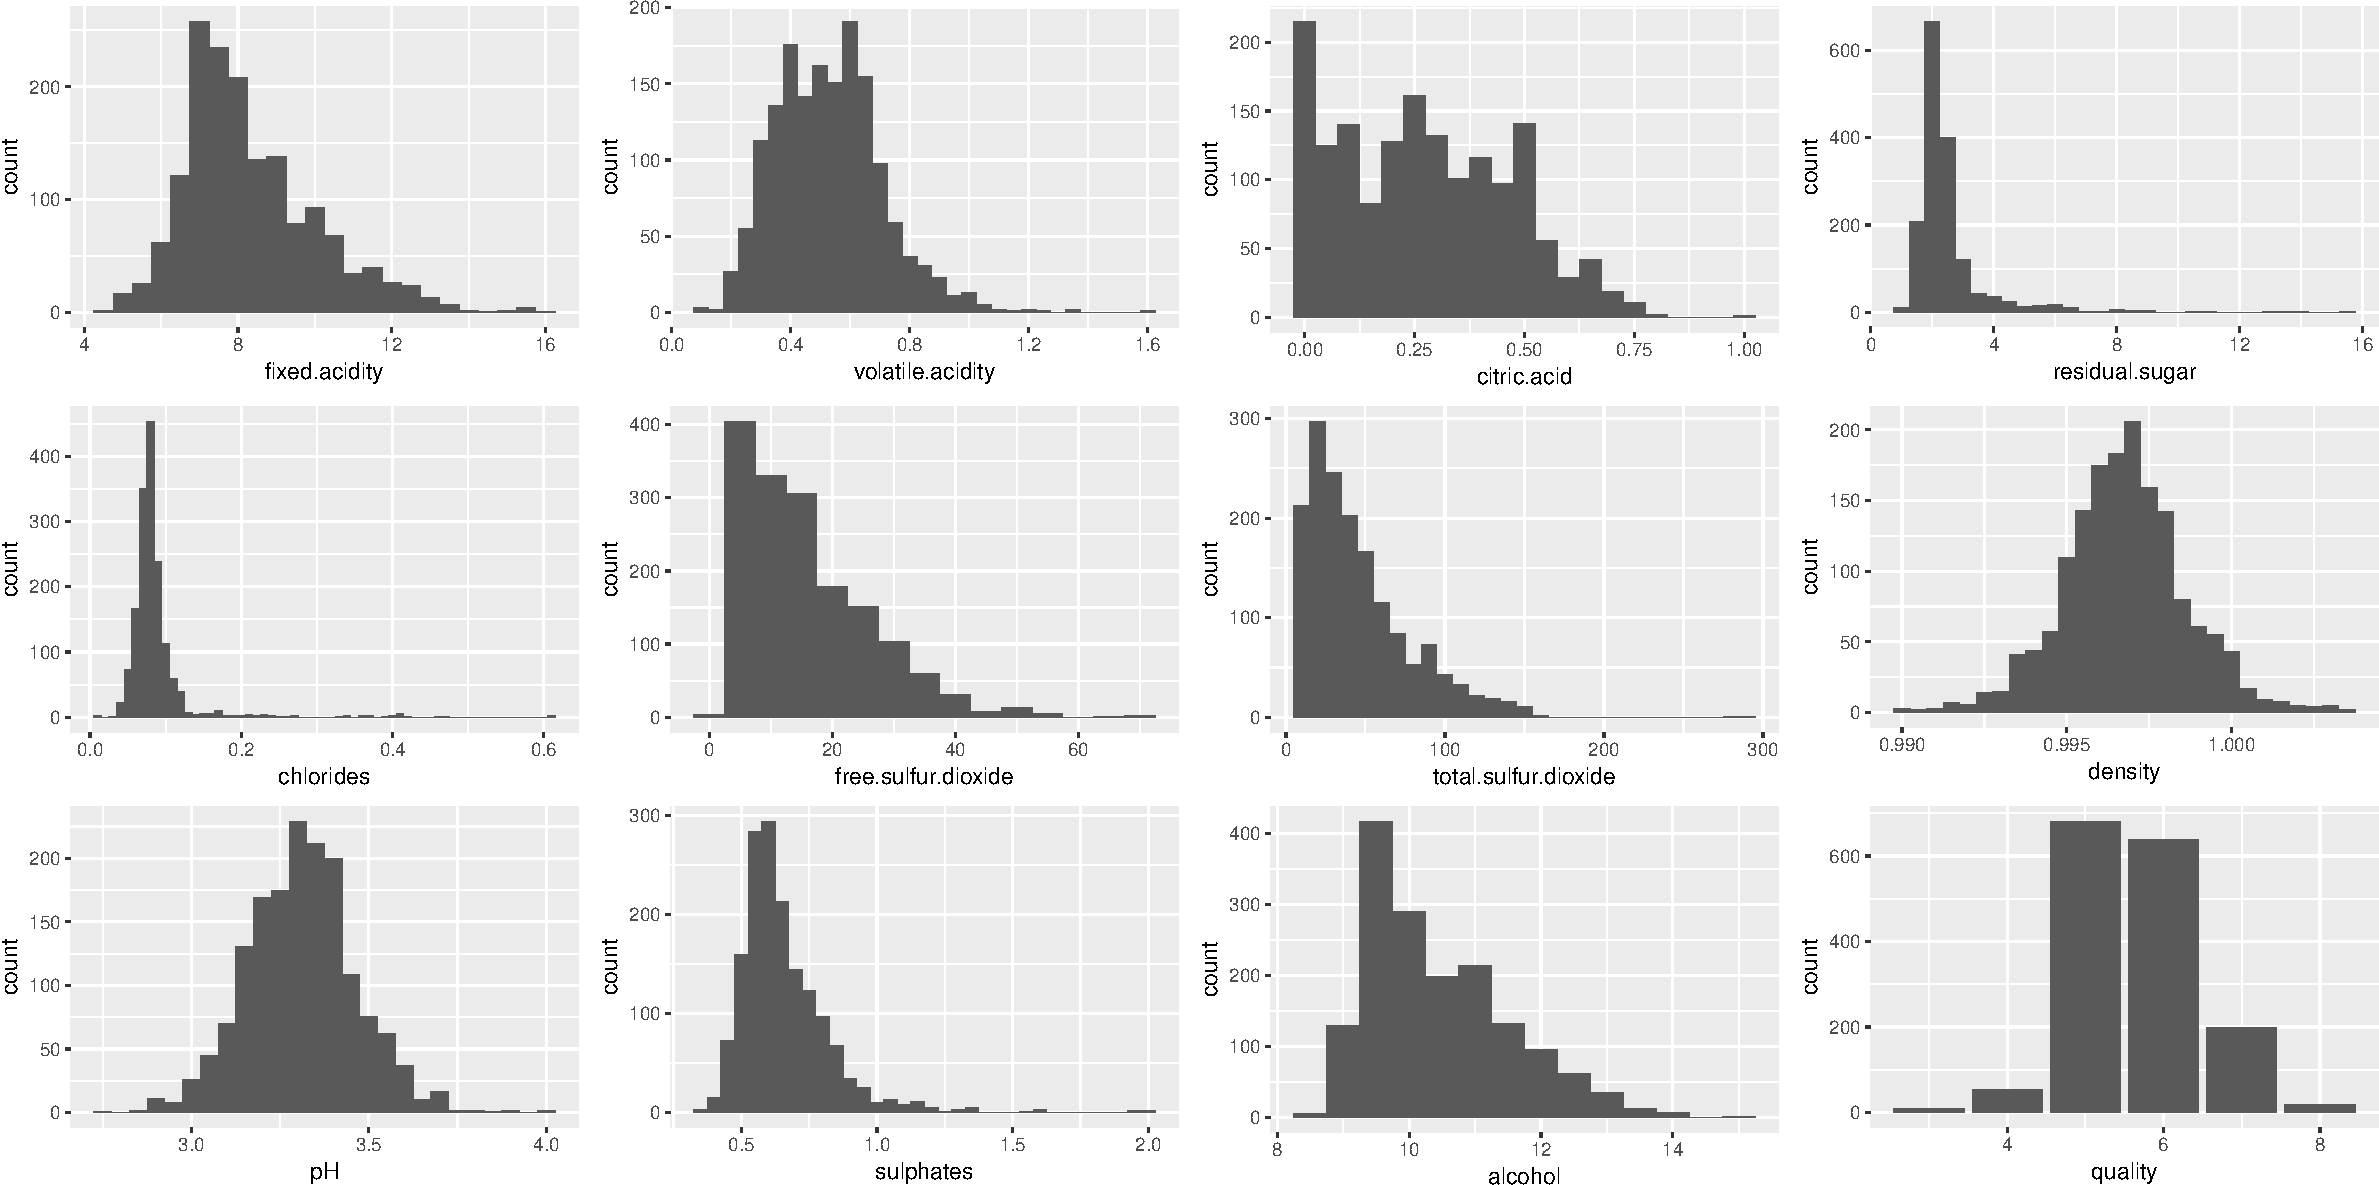
\includegraphics{Figs/Univariate_Plots_1-1.pdf}

\bibliography{P4.bib}


\end{document}
